\section{Almacenamiento de datos} \label{sec:datos}

En términos generales, la funcionalidad más relevante de la aplicación es su capacidad para registrar y recuperar datos de forma eficiente y combinar datos de múltiples fuentes para obtener información útil. En este sentido se propone un sistema de archivos compuesto por cuatro tipos principales de bases de datos, lo que, en el contexto de la ingeniería de software, se conoce como ``persistencia políglota''. El primer tipo corresponde a las bases de datos privadas del usuario, que permiten registrar: 1) contactos de personas o empresas, 2) ubicaciones como marcadores, lotes o caminos y 3) tareas agropecuarias. El segundo tipo corresponde a las bases de datos colaborativas, que consisten en colecciones de datos que se pueden generar, modificar y distribuir libremente entre usuarios y que pueden emplearse para distintos propósitos dentro del contexto del sistema, como agilizar procesos de cálculo, autocompletar formularios o simplemente consultar información. El tercer tipo de base de dato dispone de herramientas de consulta, es decir, esquemas de filtrado y búsqueda que se pueden ejecutar sobre la base de datos de tareas agropecuarias de manera que sea posible extraer información útil para el usuario. Finalmente, el cuarto tipo de base de dato contiene herramientas de cálculo, donde cada una está compuesta por un formulario para el ingreso de parámetros de entrada y una librería de fórmulas matemáticas o procedimientos lógicos para generar resultados o parámetros de salida en formato compatible con el campo correspondiente a la sección de parámetros de las tareas.

Por cuestiones de seguridad y de complejidad de implementación, el diseño actual del software no admite la edición colaborativa de las bases de datos de las herramientas de consulta y cálculo, pero es una característica que es completamente factible de incorporar al sistema para convertirlo en una plataforma que admita el intercambio de este tipo de información y de esta manera, generar un potencial mercado de conocimiento \cite{kafentzis2004}, particularmente aplicado a los negocios agropecuarios. 

A continuación se describen las características de cada tipo de base de datos, el propósito de cada una, los distintos casos de uso y potenciales aplicaciones. Finalmente se ilustran los componentes y las relaciones entre cada uno en el esquema de la Figura \ref{fig:ontologia}.

\subsection{Bases de datos privadas} \label{sec:db_priv}
% lotes, contactos -> documentos (tareas)
La aplicación cuenta con tres bases de datos locales para almacenar información privada del usuario: contactos, ubicaciones y tareas. No se emplearon sistemas relacionales para implementar estas bases de datos, para mantener flexibilidad en cuanto al formato de los datos durante el desarrollo, aunque esto se logra al costo de un menor rendimiento en materia de velocidad para búsqueda y consulta. Este esquema resulta conveniente para el caso de prototipos como lo es el desarrollo que se propone en este trabajo, pero no es la alternativa más apropiada para lograr que el producto escale manteniendo un buen rendimiento computacional en el largo plazo.

\subsection{Bases de datos colaborativas} \label{sec:ipfs}
% info gral (productos, insumos, parámetros, cultivos, etc)
El proceso de carga de datos a un sistema mediante \textit{data entry} es costoso y no garantiza la completa disponibilidad de la información que el usuario muchas veces desea manejar, por lo que en este desarrollo se optó por el empleo de una alternativa conocida como \textit{crowdsourcing} o \textit{crowd sensing}, la cual consiste en permitir la recolección de datos colaborativa y voluntaria por parte de los mismos usuarios \cite{boubiche2019}.

A modo de servicio independiente dentro de la aplicación que se detalla en este trabajo, se propone el uso de un sistema de archivos distribuido para editar de forma colaborativa y compartir datos genéricos que resulten útiles dentro de la aplicación. A continuación se listan ejemplos de bases de datos que actualmente se incluyeron en la primera versión del software y se enumeran los posibles casos de uso de cada una.

\begin{itemize}
    \item \textbf{Actividades agropecuarias}: esta base de datos sugiere una categorización u organización jerárquica de actividades. Se emplea para darle contexto a una tarea registrada por el usuario.
    \item \textbf{Propiedades de cultivos}: como peso de mil semillas, peso por metro cúbico y ángulo de reposo de granos. Esta información es útil para realizar cálculos de siembra y almacenaje de granos. También es posible incluir otras propiedades como requerimientos hídricos, o recomendaciones de producción.
    \item \textbf{Propiedades de agroquímicos}: marcas, dosis recomendadas, forma de acción, precauciones de uso, etc. Permite consultar información y autocompletar campos con nombres extensos de productos para agilizar la generación de recetas, órdenes de labor o registrar inventarios.
    \item \textbf{Requerimientos hídricos de ganado}: valores de requerimientos hídricos diarios de distintas especies y categorías de animales, lo que permite estimar aguadas como tanques y bebederos o calcular molinos y bombas de extracción de agua de pozo según cantidad de cabezas.
    \item \textbf{Modelos de molinos}: propiedades de los modelos de molinos más utilizados, entre las que aparecen diámetro de rueda, altura, diámetro de cañerías, cilindros y varillas y los resultantes valores de caudal de agua. 
    \item \textbf{Insumos para alambrados}: tipos de alambre, varillas, postes y torniquetes empleado en el cálculo de insumos para la construcción de alambrados tradicionales.
\end{itemize}    

Se espera que en el futuro los usuarios puedan consultar la disponibilidad de las distintas bases de datos según sean requeridas y que sea posible editar libremente el contenido a partir de la creación de réplicas, ya que para evitar conflicto de formatos y tipos, las bases de datos son de sólo lectura. Por este motivo, para descargar una base de datos del sistema distribuido, un usuario debe conocer el identificador de contenido (CID, por sus siglas en inglés) de la base de datos correspondiente, que se calcula a partir de una función hash. Se detallan las cuestiones técnicas referidas a la implementación de este sistema de archivos distribuido en la sección \ref{sec:comunicacion}.

\subsection{Herramientas de consulta} \label{sec:db_query}
% extracción de información de la base de datos de documentos
De forma general, se podría decir que crear una consulta para una base de datos consiste en redactar una serie de condiciones que debe cumplir cada uno de los datos del conjunto que se desea recuperar. En el caso del modelo de datos que se emplea para la base de datos de tareas agropecuarias, es posible desarrollar una gran variedad de consultas para extraer información útil. En la siguiente lista se enumeran algunos ejemplos de consultas con distinto nivel de complejidad en su lógica, que es posible aplicar para recuperar información de la base de datos de tareas.

\begin{itemize}
    \item Listar todas las labores realizadas en un mismo lote a lo largo de la última campaña, o de cualquier periodo de tiempo especificado.
    \item Obtener la suma de precipitaciones acumulada durante el año actual y comparar el valor con la media histórica anual.
    \item Calcular la cantidad de insumos o materiales totales utilizados durante cierto periodo de tiempo o en cierta ubicación.
    \item Calcular la superficie total dada a trabajar a un mismo contratista durante el último año o la cantidad de kilómetros total contratada a cierto transportista, ya sea de cereales, ganado o cualquier producto.
\end{itemize}

Estas consultas se desprenden a partir de distintos casos de usos que algunas plataformas de gestión agrícola resuelven de forma nativa. De manera similar a lo que ocurre con las bases de datos, el hecho de que exista la posibilidad de que los mismos usuarios puedan editar y compartir sus propias herramientas de consulta, permitiría generar un espacio virtual para la creación de conocimiento de gran valor para el sector agropecuario.

\subsection{Herramientas de cálculo} \label{sec:calculos}
% modelos de calculo: formularios + ecuaciones = parametros
En el contexto de la plataforma que se presenta, las herramientas de cálculo combinadas con las bases de datos permiten, en cierta manera, modelar conocimiento y compartirlo entre usuarios. El modelo de cálculo que se emplea en esta plataforma consiste en dos elementos principales: un formulario para el ingreso de variables y una librería de fórmulas o algoritmos para el cálculo de los resultados, siendo estos últimos expresados en el formato de parámetros, el cual fue formalizado en la sección \ref{sec:modelo}. Este modelo fue pensado para cubrir un amplio conjunto de herramientas de cálculo y que pueda ser utilizado por los mismos usuarios para desarrollar sus propias herramientas.

Debido a que el software propuesto aún no dispone de interfaces para la creación, distribución, búsqueda y descarga de herramientas de cálculo por parte de los usuarios, la aplicación se distribuye con una serie de herramientas de cálculo precargadas y que se enumeran en la siguiente lista junto con una breve descripción de cada una.

\begin{itemize}
    \item \textbf{Parámetros de pulverización}. Permite determinar los parámetros operativos de pulverizadoras de arrastre. Las ecuaciones fueron extraídas del trabajo presentado en \cite{criollo}.
    \item \textbf{Parámetros de siembra}. Similar al caso anterior pero aplicado a todo lo relacionado con la siembra de granos gruesos, finos y tanto convencional como directa. Basado en el trabajo presentado en \cite{campero}.
    \item \textbf{Insumos de pulverización}. Esta calculadora permite determinar la cantidad de insumos totales dados los parámetros de aplicación y la superficie a pulverizar. Estas ecuaciones también fueron tomadas del trabajo presentado en \cite{criollo}.
    \item \textbf{Merma por humedad de granos}. Permite calcular la pérdida de peso de granos durante el secado. Esta calculadora emplea la base de datos de cultivos que contiene valores de humedad aceptable para cada variedad.
    \item \textbf{Almacenaje de granos}. Esta herramienta permite determinar el peso almacenado en silos tipo torre de base plana o cónica y galpones a partir de las dimensiones. Esta calculadora emplea la base de datos de cultivos para obtener los valores de ángulo de reposo de los distintos granos.
    \item \textbf{Dimensionamiento de aguadas}. Esta calculadora permite estimar volúmenes de aguadas y tamaño de molinos requeridos según la cantidad de cabezas de ganado. Para agilizar los cálculos, se puede emplear una base de datos de requerimientos hídricos de las distintas especies y categorías de animales.
\end{itemize}

\begin{figure}[t]
    \centering
    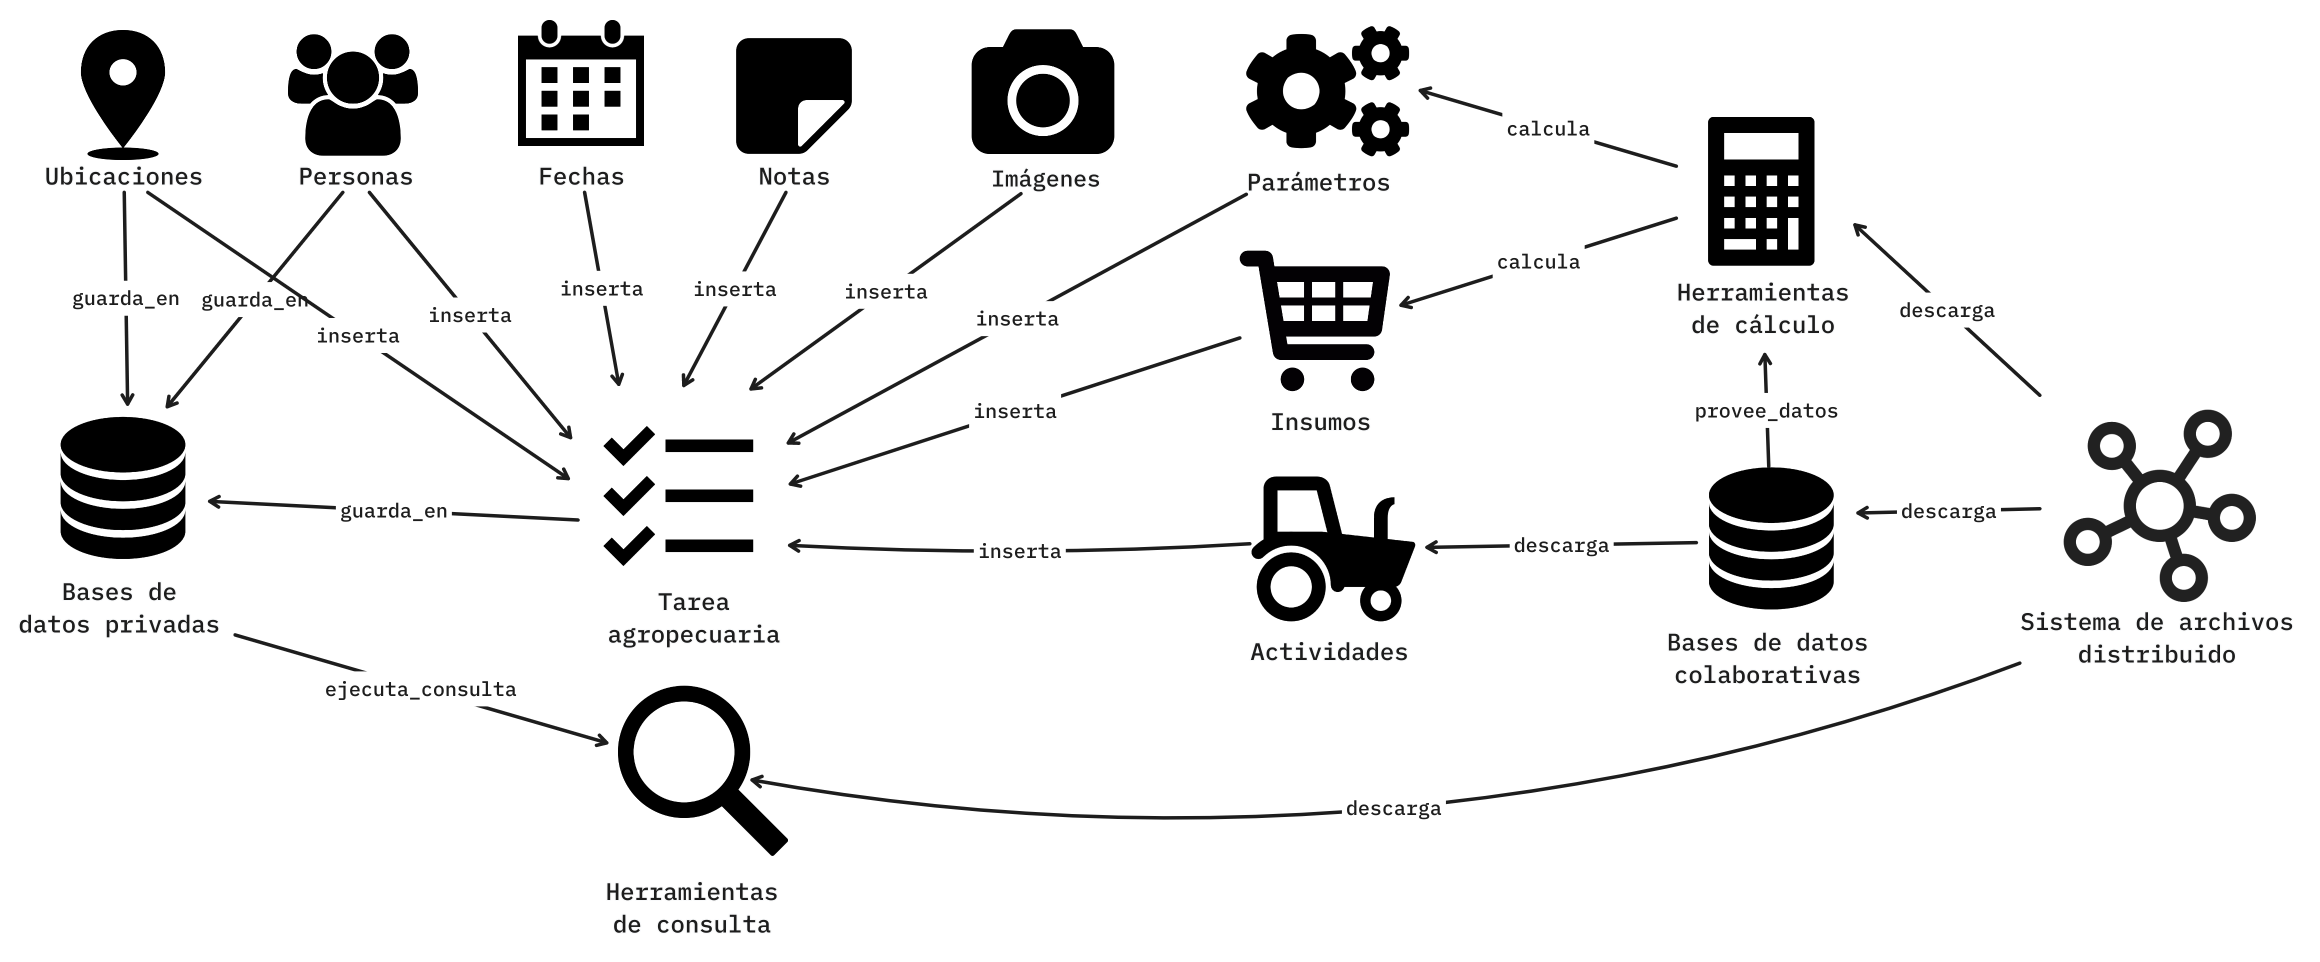
\includegraphics[width=\textwidth]{imagenes/ontologia2_lowres.png}
    \caption{Componentes del sistema y relaciones.} \label{fig:ontologia}
\end{figure}

